\section{Design}
Conceptualizing a single ETL process as an entity of type \textit{Task}, that is, the ``extraction, transformation and loading of data from a source to destination'', provides a focal point on which the nETL software can be architected. \textit{Task} instances are created by a constructor that takes a configuration object (loaded from a JSON file) as an object. Each task-instance is referenced by a singleton object created on app instantiation - the \mintinline{text}{taskManager}.

Starting the long-running nETL process comprises instantiating the \mintinline{text}{taskManager} singleton. This object provides a CLI (command line interface) to facilitate user interactions. Via the CLI, users can interact with \mintinline{text}{taskManager} to register different ETL components, start/stop tasks, configure application options such as log output path, etc.

The relationship between the \mintinline{text}{taskManager} singleton, \mintinline{text}{task} instances, and components is shown in Figure \ref{fig-nETL}. ETL components comprise modules that adhere to the Module interface and that accept a TaskConfig object as a paramater on instantiation. As such modules are paired with configuration objects as shown in the coloured blocks. An ETL task comprises the following steps:

\begin{itemize}
    \item Loading all component modules required for a specific task into the nETL runtime
    \item Loading a configuration object that directs how each module should perform into the nETL runtime
    \item The runtime engine reads the configuration object, and runs the components as directed
\end{itemize}

\begin{figure}[H]
    \centering
    \begin{mdframed}
        \centering
        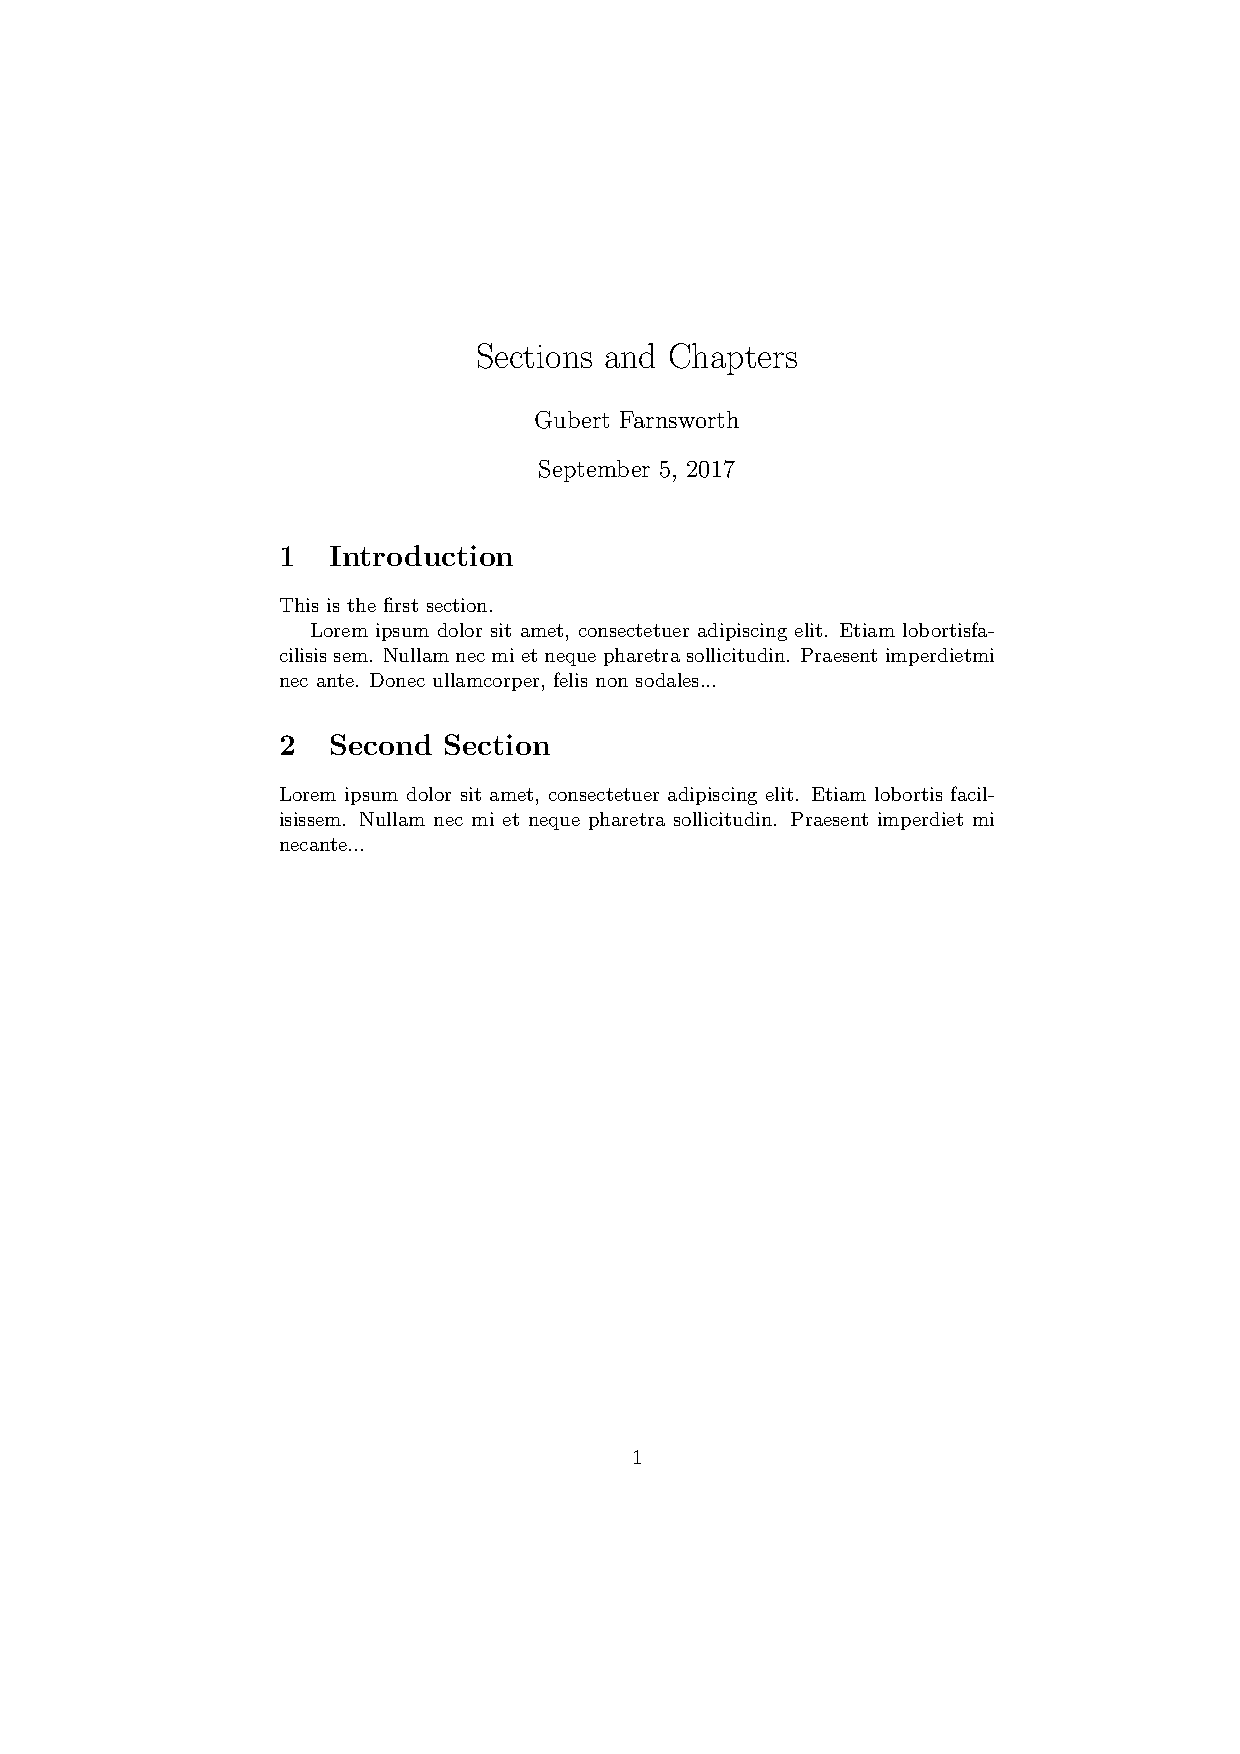
\includegraphics[scale=0.39]{./resources/figures/netl.png}
    \end{mdframed}
    \caption[nETL Architecture]{\textbf{Figure \ref{nETL}: nETL Architecture.} \textit{nETL} is an ETL framework designed to host user-created \textit{Modules} to define \textit{extraction}, \textit{transformation} and \textit{loading} processes. \textit{Modules}, shown in the colored boxes, consist of two parts: a configuration object (a JSON object) and a function that adheres to the specified contract. On startup the \textit{nETL} framework loads modules via the operations via a function made available by the main class. The modules are then cached in main memory by the \textit{nETL} process. A user can then interact with the TaskManager class to create a new task via loading a JSON configuration that makes use of a particular \textit{Module}. Tasks consist of an \textit{Extraction module} configuration, several \textit{Transformation module} configurations and a \textit{Load} configuration. Because modules are created and defined by users, as well as the order in which modules are executed, input/output contracts are also defined by the user, and as such \textit{ETL} processes are infinitely configurable.}
    \label{nETL}
\end{figure}